\PassOptionsToPackage{table,xcdraw}{xcolor}

%% For double-blind review submission, w/o CCS and ACM Reference (max submission space)
\documentclass[acmsmall,nonacm]{acmart} 
\pagestyle{plain} % removes running headers

\bibliographystyle{ACM-Reference-Format}
%\citestyle{acmauthoryear}   %% For author/year citations

\usepackage{url}
\usepackage{amsmath}
\usepackage{amsfonts}
\usepackage{amssymb}
\usepackage{listings}
\usepackage{color}
\usepackage{graphicx}

%% https://github.com/nickgian/thesis/blob/master/lstcoq.sty
\usepackage{color}

\definecolor{ltblue}{rgb}{0,0.4,0.4}
\definecolor{dkblue}{rgb}{0,0.1,0.6}
\definecolor{dkgreen}{rgb}{0,0.35,0}
\definecolor{dkviolet}{rgb}{0.3,0,0.5}
\definecolor{dkred}{rgb}{0.5,0,0}

% lstlisting coq style (inspired from a file of Assia Mahboubi)
%
\lstdefinelanguage{Coq}{ 
%
% Anything betweeen $ becomes LaTeX math mode
mathescape=true,
%
% Comments may or not include Latex commands
texcl=false, 
%
% Vernacular commands
morekeywords=[1]{Section, Module, End, Require, Import, Export,
  Variable, Variables, Parameter, Parameters, Axiom, Hypothesis,
  Hypotheses, Notation, Local, Tactic, Reserved, Scope, Open, Close,
  Bind, Delimit, Definition, Let, Ltac, Fixpoint, CoFixpoint, Add,
  Morphism, Relation, Implicit, Arguments, Unset, Contextual,
  Strict, Prenex, Implicits, Inductive, CoInductive, Record,
  Structure, Canonical, Coercion, Context, Class, Global, Instance,
  Program, Infix, Theorem, Lemma, Corollary, Proposition, Fact,
  Remark, Example, Proof, Goal, Save, Qed, Defined, Hint, Resolve,
  Rewrite, View, Search, Show, Print, Printing, All, Eval, Check,
  Projections, inside, outside, Def},
%
% Gallina
morekeywords=[2]{forall, exists, exists2, fun, fix, cofix, struct,
  match, with, end, as, in, return, let, if, is, then, else, for, of,
  nosimpl, when},
%
% Sorts
morekeywords=[3]{Type, Prop, Set, true, false, option},
%
% Various tactics, some are std Coq subsumed by ssr, for the manual purpose
morekeywords=[4]{pose, set, move, case, elim, apply, clear, hnf,
  intro, intros, generalize, rename, pattern, after, destruct,
  induction, using, refine, inversion, injection, rewrite, setoid_rewrite, congr,
  unlock, compute, ring, field, fourier, replace, setoid_replace, fold, unfold,
  change, cutrewrite, simpl, have, suff, wlog, suffices, without,
  loss, nat_norm, assert, cut, trivial, revert, bool_congr, nat_congr,
  symmetry, transitivity, auto, split, left, right, autorewrite},
%
% Terminators
morekeywords=[5]{by, done, exact, reflexivity, tauto, romega, omega,
  assumption, solve, contradiction, discriminate},
%
% Control
morekeywords=[6]{do, last, first, try, idtac, repeat},
%
% Comments delimiters, we do turn this off for the manual
morecomment=[s]{(*}{*)},
%
% Spaces are not displayed as a special character
showstringspaces=false,
%
% String delimiters
morestring=[b]",
morestring=[d]’,
%
% Size of tabulations
tabsize=3,
%
% Enables ASCII chars 128 to 255
extendedchars=false,
%
% Case sensitivity
sensitive=true,
%
% Automatic breaking of long lines
breaklines=false,
%
% Default style fors listings
basicstyle=\small,
%
% Position of captions is bottom
captionpos=b,
%
% flexible columns
basewidth={2em, 0.5em},
columns=flexible,
%
% Style for (listings') identifiers
identifierstyle={\ttfamily\color{black}},
% Style for declaration keywords
keywordstyle=[1]{\ttfamily\bfseries\color{dkviolet}},
% Style for gallina keywords
keywordstyle=[2]{\ttfamily\bfseries\color{dkgreen}},
% Style for sorts keywords
keywordstyle=[3]{\ttfamily\bfseries\color{ltblue}},
% Style for tactics keywords
keywordstyle=[4]{\ttfamily\color{dkblue}},
% Style for terminators keywords
keywordstyle=[5]{\ttfamily\color{dkred}},
%Style for iterators
%keywordstyle=[6]{\ttfamily\color{dkpink}},
% Style for strings
stringstyle=\ttfamily,
% Style for comments
commentstyle={\ttfamily\itshape\color{dkgreen}},
%
%moredelim=**[is][\ttfamily\color{red}]{/&}{&/},
literate=
    {fun}{{\color{dkgreen}{$\lambda\;$}}}1
    {bool}{{$\mathbb{B}$}}1
    {nat}{{$\mathbb{N}$}}1
    {Vforall2}{Vforall2}1 % quick workardoun to avoid partial replacement of 'forall' in identifier
    {nat\_equiv}{nat\_equiv}1 % quick workardoun to avoid partial replacement of 'nat' in identifier
    {forall}{{\color{dkgreen}{$\forall\;$}}}1
    {exists}{{$\exists\;$}}1
    {<-}{{$\leftarrow\;\;$}}1
    {=>}{{$\Rightarrow\;\;$}}1
    {==}{{\texttt{==}\;}}1
    {==>}{{$\Longrightarrow\;\;$}}1
%    {:>}{{\texttt{:>}\;}}1
    {->}{{$\rightarrow\;\;$}}1
    {<-->}{{$\longleftrightarrow\;\;$}}1
    {<->}{{$\leftrightarrow\;\;$}}1
    {<==}{{$\leq\;\;$}}1
    {\#}{{$^\star$}}1 
    {\\o}{{$\circ\;$}}1 
%    {\@}{{$\cdot$}}1 
    {\/\\}{{$\wedge\;$}}1
    {\\\/}{{$\vee\;$}}1
    {++}{{\texttt{++}}}1
    {~}{{\ }}1
    {¬}{{$\lnot$}}1     % this does not work
    {\@\@}{{$@$}}1
    {\\mapsto}{{$\mapsto\;$}}1
    {\\hline}{{\rule{\linewidth}{0.5pt}}}1
%
}[keywords,comments,strings]

\lstnewenvironment{coq}{\lstset{language=Coq}}{}

% pour inliner dans le texte
\def\coqe{\lstinline[language=Coq, basicstyle=\small]}
% pour inliner dans les tableaux / displaymath...
\def\coqes{\lstinline[language=Coq, basicstyle=\scriptsize]}

%%% Local Variables: 
%%% mode: latex
%%% Local IspellDict: british
%%% TeX-master: "main.tex"
%%% End: 
\usepackage{booktabs} 
\usepackage{subcaption}

\newcommand{\N}{\mathbb{N}}
\newcommand{\asnc}{\texttt{asn1c}}
 
\usepackage{amsmath}
\usepackage{amssymb}
\usepackage{latexsym}
\usepackage{relsize}
\usepackage{xcolor}
\usepackage{color}
\usepackage{mathtools}
\usepackage{enumitem}

%\usepackage{multicol}

\lstset{
  basicstyle=\ttfamily\small,
  frame=tb, % draw a frame at the top and bottom of the code block
  tabsize=4, % tab space width
  showstringspaces=false, % don't mark spaces in strings
  numbers=left, % display line numbers on the left
  commentstyle=\color{green}, % comment color
  keywordstyle=\color{blue}, % keyword color
  stringstyle=\color{red}, % string color
  % identifierstyle=\color{grey},
}

\lstdefinelanguage{diff}{
    morecomment=[f][\color{diffstart}]{@@},
    morecomment=[f][\color{diffincl}]{+},
    morecomment=[f][\color{diffrem}]{-},
  }

\begin{document}

\title{Work-in-Proress: Formally-Verified ASN.1 Protocol C-language Stack}

\author{Nika Pona}
\affiliation{
  \institution{Digamma.ai}
}
\email{npona@digamma.ai}
\author{Vadim Zaliva}
\affiliation{
  \institution{Carnegie Mellon University}
  \department{ECE}
}
\email{vzaliva@cmu.edu}

\begin{abstract}
We describe our approach and progress in verification of an exsiting mature open-source ASN.1 compiler ASN1C using the Coq proof assistant. 
\end{abstract}

\maketitle

\tableofcontents

\section{Introduction}

\subsection{Background}

The pervasively deployed and widely adopted ASN.1 (``Abstract Syntax
Notation One'') \cite{ASN1Intro} joint standard of the International
Telecommunication Union (ITU-T) and the International Organization for
Standardization (ISO/IEC) provides an essential interface description
language for defining data structures for serialized and deserialized
cross-platform data exchange, broadly used in telecommunications,
computer networking, the Internet, and cryptography. ASN.1 is
vitally relied upon by core aspects of the Internet infrastructure and
Internet applications such as telephony, enterprise computing,
utilities, finance, military, security, digitally-controlled
infrastructure, transportation, medical systems, and commercial cloud
computing.

An example ASN.1 module that describes an X.509-like public key certificate
is shown in Listing~\ref{lst:asnex}.
Such certificates are used by every browser to access HTTPS web sites.
The original ASN.1 definition for the X.509 standard takes about 1000 lines
of ASN.1 and is not practical to include into this report. Using ASN.1 language one can define data structures that use ASN.1 {\it primitive types}, such as INTEGER, BOOLEAN, OBJECT IDENTIFIER etc, and {\it constructed types}, such as SEQUENCE (OF), SET (OF), CHOICE (OF).

\begin{lstlisting}[language=C,label=lst:asnex,
  caption={ASN.1 example of X.509 certificates, adapted for brevity}]
X509 DEFINITIONS ::= BEGIN

  Certificate  ::=  SEQUENCE  {
    tbsCertificate       TBSCertificate,
    signatureAlgorithm   AlgorithmIdentifier,
    signature            BIT STRING
  }

  TBSCertificate  ::=  SEQUENCE  {
     version         [0]  INTEGER,
     serialNumber         INTEGER,
     signature            AlgorithmIdentifier,
     issuer               Name,
     subject              Name,
     subjectPublicKeyInfo SubjectPublicKeyInfo,
  }

  SubjectPubicKeyInfo ::= SEQUENCE {
    algorithm           AlgorithmIdentifier,
    subjectPublicKey    BIT STRING
  }

  AlgorithmIdentifier ::= SEQUENCE {
    algorithm           OBJECT IDENTIFIER
  }

  Name ::= SEQUENCE OF SET OF SEQUENCE {
    type                OBJECT IDENTIFIER,
    value               ANY DEFINED BY type
  }

END
\end{lstlisting}


A typical ASN.1 stack comprises of a \textit{compiler} which parses
ASN.1 syntax definitions as shown in the Listing~\ref{lst:asnex} and
produces either a source code of a specialized protocol encoder and
decoder for this data or a runtime data for a parametric protocol
encoder and decoder.

However, the ASN.1 standard \cite{ASN1Intro} is large and complex:
currently, it comprises twelve sub-standards spanning 862 pages
supplemented by additional pages of corrigenda\cite{ASN1Intro}. This opens
a door for many potential software bugs and malicious exploits.
  
\subsection{Motivation}

Proliferating embedded and user computing devices are implementing
vast numbers of essential functions and applications, all of which
exchange data using ASN.1. The resulting interconnected communicating
systems are becoming riskier, less stable, less reliable, and
potentially dangerous. Disruption of the ASN.1 based communications
could threaten the functioning of the critical infrastructure our
society relies upon.


The Computer Vulnerabilities and Exposures (CVE) database
\cite{CVE} lists critical ASN.1-related bugs found each year in
the existing systems, and there have already been noteworthy exposures
\cite{OpenSSLMemoryCorruption} that although not as dire to security as first feared
\cite{ASN1Flaw} clearly spell out a first awareness of the vast risk and
exposure. We analyzed the last 4 years of ASN.1-related issues
reported in Computer Vulnerabilities and Exposures (CVE) database
\cite{CVEaddon}. Among vulnerabilities studied were CVEs for various
software and hardware products and vendors, including \textit{Apple},
\textit{axTLS}, \textit{Botan}, \textit{Bounty Castle},
\textit{librcrypto++}, \textit{libtasn}, \textit{LibTomCrypt},
\textit{Linux Kernel}, \textit{MatrixSSL}, \textit{Mozilla NSS
  (Firefox)}, \textit{Objective Systems}, \textit{OpenSSL},
\textit{PolarSSL}, \textit{RSA BSAFE}, \textit{Samba},
\textit{Samsung}, \textit{Snapdragon}, \textit{strongSwan}, and
\textit{Wireshark}. It was found that 39 out of 52 problems analyzed
were related to memory safety, 6 related to stack and heap bounds
checking, and 3 related to issues caused by applications accepting not
well-formed ASN.1 input. Having proved just six formal properties
would have prevented 49 out of 52 vulnerabilities, that is, more than
90\% of reported vulnerabilities\footnote{See Appendix B for more details}.


\subsection{Our approach}

Systems and methods to date either (a) are automatically tested but not
formally verified (b) use verification approaches which rely on
automatic extraction from executable specifications (for example
involving network stack synthesis \cite{VNSSforSel4}, optimizing compilers
\cite{CompCert}, cryptographic libraries \cite{HACL}, and
encoder/decoders \cite{Narcissus}), or (c) apply a form of formal
verification which only proves partial correctness properties (partial
verification of NAT stack only proving parts of DPDK are specification
compliant \cite{NAT}, partial verification of Linux kernel TCP
implementation with 55\% line coverage and 92\% protocol coverage
\cite{NSDI}). Consequently, (a) and (c) do not provide sufficient
correctness guarantees, while (b) is often impractical due to poor
performance and compatibility limitations. In contrast, we pursue a
far deeper and comprehensive verification approach to performance and
portability and seek to prove actual industrial-level C-code
implementation.

As shown in Figure~\ref{fig:components} the project begins with ITU-T
standard document in the form of human-readable text. We will manually
convert it into formal specification (H.SPEC). This is high-level
specification (in Coq) which describes the correspondence between data
types (such as integers) and packet octets data layout. This
specification is one of the outputs of this project and has a value of
its own.

\begin{figure}[h!]
  \centering
  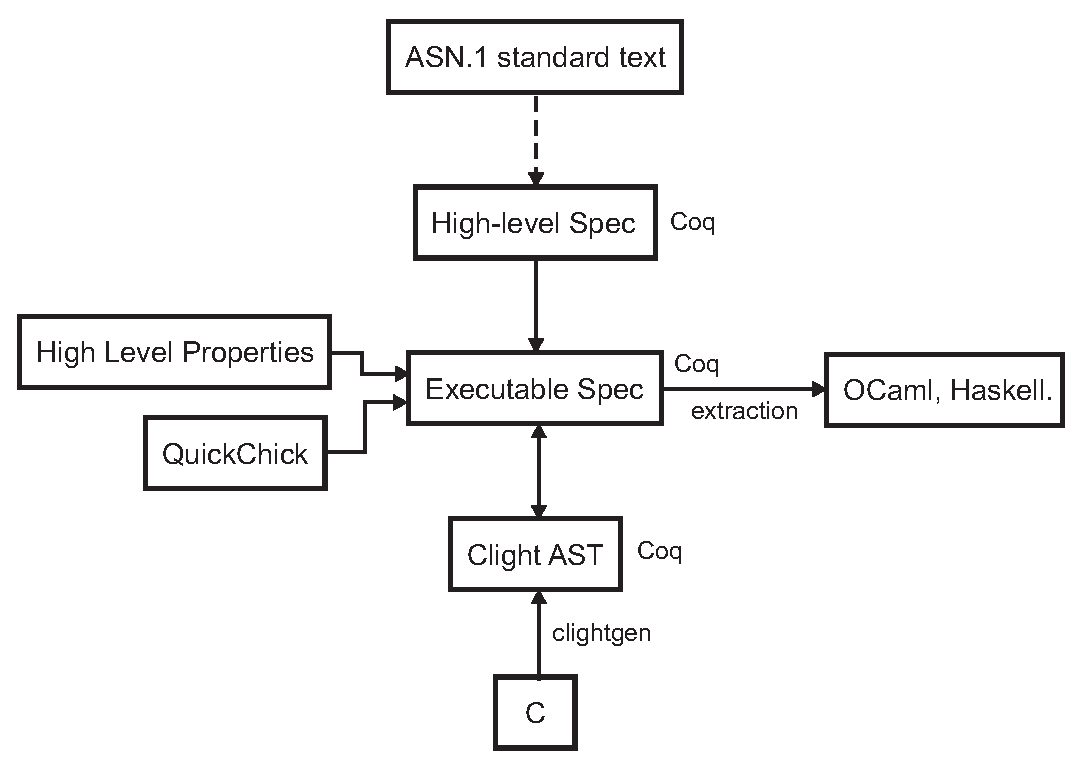
\includegraphics[width=10cm]{VerificationArchitectureDiagram.eps}
  \caption{Verification Architecture}
  \label{fig:components}
\end{figure}

Next level of refinement is Executable Specification (E.SPEC). Also
written in Coq it describes ``encoder'' and ``decoder'' for each type
as a pair of pure functions. We will prove that the Executable
specification encodes and decodes bytes are in conformance to High-Level
specification.

``High-Level Properties'' like termination, computation complexity and
memory safely could be proven based on executable specification. They
are shown as ``High Level'' box on the left in the Figure 1. The executable spec
contains enough information to \textit{extract} a fully functional
encoder program in languages supported by Coq extraction mechanism
(e.g. OCaml and Haskell) \cite{Extraction}. Such a possibility is shown with the box
on the right in Figure~\ref{fig:components} although we do not plan to
pursue it yet. This approach others often take and it has some
drawbacks. However, it should be noted that all the work we will do up
to and including Executable Spec is compatible with this approach and
if needed we can revisit it. For example, in case if we need to
generate ASN.1 stack for special platforms where OCaml code opens some
additional opportunities for parallelization, optimization or
integration. One example of such platforms could be MirageOS
\cite{MirageOS} which is an OCaml-based unikernel.

The box at the left marked \textit{QuickChick} represents another
possibility we might not pursue immediately. It is using randomized
property-based automated testing based on on an executable
specification to further verify its correctness. This work could be
done using QuickChick \cite{QuickChick} in Coq. It is also could be used
to generate a test-suite for extracted code.

At the bottom of Figure 1 is a box labeled ``C'' which represents the
existing C code of ASN1C compiler. Using an automated conversion
provided by the \texttt{clightgen} tool within the CompCert C compiler
\cite{CompCert} we will convert this to an Abstract Syntax Tree (AST)
\cite{AST} (labeled ``C.AST'' in Figure 1) rendered in a subset
of C-language called Clight \cite{Mechanized} that is recognized by Coq. More specifically,
CompCert converts C ``concrete syntax'' to ``abstract'' Clight
syntax. The resulting Clight program is just a reification of the
original C program in Coq, retaining the overall structure and
preserving the semantics; Clight is further assigned formal semantics
by CompCert that can be used to further ``reason about'' (interrogate
and analyze) programs within Coq.

Finally, as the most critical (and laborious) step of the project, we
will prove that semantics of Clight
translation for each given function corresponds to executable
specification (E.SPEC). This will guarantee that the C program behaves exactly
as the executable spec.

Hence, the formal certification of correctness will comprise the following
three elements:

\begin{enumerate}[label=(\alph*)]

\item Formal specification of X.509 ASN.1 subset, which can be examined.

\item Proofs of semantic equivalence between the C code and the
  specification (in Coq Proof Assistant \cite{Coq}). From such
  proofs, Coq can generate a ``certificate'' which is a program in a
  formal language based on the Calculus of Inductive Constructions
  (``CIC'') \cite{CIC}. The ``certificate'' allows 3rd party
  validation of proofs which have been developed in Coq. The Calculus
  of Inductive Constructions (``CIC'') is a small and mathematically
  well-defined formal language that serves as the underlying formal
  system of Coq. The generated certificate is automatically validated
  by the relatively small Coq kernel. Although a fraudulent
  certificate could hypothetically be created, it will not pass
  validation when submitted to the Coq kernel. The resulting outcome
  limits the trust need to trusting the small CIC formal language and
  the small Coq kernel.

\item Proofs of additional high-level properties such as memory safety
  and termination.

\end{enumerate}
  

Element (b) ensures a bug-free standard-compliant implementation, and
element (c) provides further guarantee that it could not be exploited
in penetration or denial of service attacks.

Additionally, our (modified) version of ASN1C could be compiled with
the certified CompCert compiler \cite{CompCert} to extend correctness
guarantees through all levels down to machine code. This will provide state-of-the-art high
assurance suitable for mission-critical systems. Further, since formal
verification will be layered atop of a widely used ASN.1 stack, it
could be immediately offered to current users. This will make it attractive to new users who require higher
assurance levels than current non-verified implementations provide.

\section{Preliminary work}

\subsection{Verifying floating-point numbers encoding}

As a first estimate of the difficluties associated with
verifying ASN.1-related programs, we wrote
formal specification of an encoder-decoder pair for a small, but
particularly error-prone subset of the standard - floating-point numbers. The development is available on github \cite{asn1fpcoq}.
Our first approach was relatively straightforward: define types
representing ASN.1-encoded data in Coq, provide functions for converting
between representations and prove that they operate correctly. In particular, we proved the roundtrip property for the defined encoders/decoders.

Although providing guarantees of correctness, this technique had major disadvantages.
First of all, our definitions, being written in pure Coq, had only one
connection to the real world - through automatic code extraction.
This immediately comes with a set of problems:

\begin{itemize}
\item Writing a new implementation in Coq does not produce any improvement in pre-existing widely-used implementations
\item Automatic code extraction does not provide sufficient correctness guarantees
\item Extracted code generally runs much slower than its counterparts implemented in other languages
\item Extracted code might not be compatible with or viable in some real-world use-case scenarios
\end{itemize}

However, this attempt allowed us to home in on what approaches
to verfication were viable and improve our effort estimates. Moreover, we tested specification and proving techniques which will be useful for us in the future.

\subsection{Verifying simple  \texttt{asn1c} function}

To estimate an effort required to formally verify C code and to
experiment with various verification strategies we decided to try to
verify a small function from an existing ASN.1 compiler. We chose
function \texttt{asn\_strtoimax\_lim(const char *str, const char **end, intmax\_t *intp)} from \texttt{asn1c} compiler.
The function is relatively simple, but at the same time uses many
features of C that make verifying imperative programs
challenging. \emph{XER} decoding functions for \emph{INTEGER},
\emph{OBJECT-IDENTIFIER} and \emph{RELATIVE-OID} types (and hence all
constructed types that use these primitive types) critically depend on
this function.

The only specification provided was the following comment in the
source code. Additional specification details have to be inferred from
the source code and usage examples.

\begin{quote}
 { \it Parse the number in the given string until the given *end position,
 returning the position after the last parsed character back using the
 same (*end) pointer.
 WARNING: This behavior is different from the standard strtol/strtoimax(3). }
\end{quote}

Full source code of the function is included in the Appendix~\ref{sec:stritomax}.

\subsubsection{Bugs}

Despite that fact that this function lineage could be traced back 15
years, and it being a part of mature, well-tested ASN.1 compiler used in
many production systems during our formal verification exercise we
found three bugs in the current implementation. These bugs were never
reported before and passed all human code reviews, unit, and fuzzying
tests. The following bugs were reported to product developers,
acknowledged and promptly fixed:
  
\paragraph{Negative range bug}

When we go beyond allowed \textit{int} range, a wrong result is given
for some inputs. For example, assuming we are working on a 8-bit
system and the maximum signed integer value is 127, parsing the input
string \texttt{``-1281''} produces the result
\emph{ASN\_STRTOX\_OK} (meaning the conversion was succesfull) with the value -127 instead of expected
\emph{ASN\_STRTOX\_ERROR\_RANGE} (meaning the number to be converted is out of integer range). This happens whenever the input
string represents a number smaller than \texttt{MIN\_INT}, due to the
fact that absolute value of \texttt{MIN\_INT} is greater than
\texttt{MAX\_INT}, thus negative number cannot be treated as
$\mathrm{value}\times\mathrm{sign}$ when $\mathrm{value}$ is
represented as \textit{int}. The bug was filed and promptly fixed by
developers.

\paragraph{Memory store bug}

Another bug we discovered was related to potentially overlapping
memory areas pointed by argument pointers. Under some circumstances
the value of the \texttt{end} pointer parameter is treated as a part
of the input data and the resulting error value could be
incorrect. This bug could never occur if the function is always called
with non-overlapping pointer arguments. However this could be viewed
as an implicit pre-condition which should be part of the function's
specification.

\paragraph{Specification Ambiguity}

After addressing the two bugs we discovered we were able to
successfully verify that the function finally corresponds to the
specification we wrote for. However, it was noticed the following
behavior: For input \texttt{``a''} it stores value 0 (same behaviour as on input \texttt{``0''}) and returns
{\color{green}\texttt{ASN\_STRTOX\_EXTRA\_DATA}} (same behaviour as on
input \texttt{``0a''}), which was probably unintended by authors.
  
\subsubsection{Direct operational semantics proof}

First we formulated functional correctness and proved it using
big-step operational semantics of \textit{C light}, defined in
\textit{Compcert}. In this proof we used pure-function
re-implementation in Coq: \texttt{asn\_strtoimax\_lim : addr $\rightarrow$
  addr $\rightarrow$ addr $\rightarrow$ option
  asn\_strtoimax\_lim\_result} as an intermediate specification.

This function took addresses as inputs and operated on memory using
\texttt{load} and \texttt{store} operations from \textit{CompCert's}
memory model, while calculating the resulting machine integer
value. The proof went by induction on the distance between input
pointers and the main difficulty apart trying to prove a faulty
program (that's when we discovered two bugs) was operational semantics
control flow minuities and machine arithmetic proofs. However, only a
couple of lemmas about the specification were needed and proofs of different cases were very repetitive. Since functional
and memory specification were intertangled it was more difficult to
read the specification and make sure it was correct, hence we missed the specification ``bug'' mentioned above. 

\subsubsection{Proof using VST}

The \textit{Verified Software Toolchain} \cite{VST} offered
solutions to problems we encountered while doing direct opertational
semantics proof: it has good automation of control flow, some
automation for machine arithmetic, and clearly separates functional
and memory-related parts of the specification. It also provides a
uniform way of stating functional correctness and memory
safety, so reduces the chances of having the wrong specification. Proofs here are done using \textit{Hoare} and \textit{separation}
logic implemented in Coq, which are proven to be sound with respect to operational
semantics of CompCert. Similarly as before, we rely on C light syntax and semantics. VST has tactics that can solve simple entailments in these
logics, however, they were not powerful enough to significantly reduce
the overall proof effort. In fact, with respect to memory safety specifications,
direct operational semantics proof was shorter and more
straightforward. However, this problem can be solved by improving the existing tactics and fine-tuning the specification style, so in the end we find this approach more vible for a large project.

\paragraph{Specification layers} On this simple example we tested our architecture from Section 1.3. First we have a high-level specification of this function in declarative, relational style. Each constructor corresponds to a return message (state) and stores value and the number of iterations of the function (used to store the result in memory). Such specification can be easily examined and refined.

 \begin{lstlisting}[language=Coq]

(* Relation between input string, value, index an asn_strtox_result_e message *)
  Inductive asn_strtoimax_lim : list byte -> Z -> Z -> asn_strtox_result_e -> Prop :=
  (* Invalid data encountered *)
  | ERROR_INVAL:
      asn_strtoimax_lim nil 0 0 ERROR_INVAL
  (* More data expected (e.g. "+") *)
  | EXPECT_MORE : forall ls c,
      ls = [c]  ->
      is_sign c = true ->
      asn_strtoimax_lim ls 0 1 EXPECT_MORE
 (* Non-digit encountered *)
  | EXTRA_DATA : forall c ls z i,
      asn_strtoimax_lim ls z i OK ->
      is_digit c = false -> 
      asn_strtoimax_lim (ls ++ [c]) z i EXTRA_DATA
   ...    
  \end{lstlisting}

Next level is executable specification \texttt{Z\_of\_string} which we prove equivalent to the relational specification, but which we can extract to Coq and which is easier to use in the proof. Here we experimented with two approaches. The function below can serve as a functional specification for \texttt{asn\_strtoimax\_lim} and is not that different from the relational spec.

 \begin{lstlisting}[language=Coq]
Fixpoint Z_of_string_loop (s : list byte) (val index : Z) (b : bool) := 
    match s with 
    | [] => {| OK; val; index |}
    | c :: tl => 
      if is_digit c
      then let val' := app_char b val c in 
           if bounded val'
           then Z_of_string_loop tl val' (index + 1) b
           else {| ERROR_RANGE; val'; index; |}      
      else {| EXTRA_DATA; val; index; |}              
    end.

Definition app_char (b : bool) v c := 
  if b then v * 10 + (Z_of_char c) 
       else v * 10 - (Z_of_char c).
 \end{lstlisting}

Since \texttt{Z\_of\_string} has different structure from \texttt{asn\_strtoimax\_lim}, the proof required many lemmas to connect functional spec to the C code and complicated the loop invariant. We found that it is more effective to separate the functional aspect of the proof from C-proof as much as possible to allow for more automation in the proof of C function correctness. Thus we defined another intermediate spec \texttt{Z\_of\_string\_C}, which is basically functional re-implementation of the C function, alike the one we used in operational semantics proof, but without mentioning memory and operation on abstract \texttt{Z} type and not machine integers. Then we prove that texttt{Z\_of\_string\_C} is equivalent to \texttt{Z\_of\_string}, which is a simple functional correctness proof that allows to eliminate the need for additional lemmas in the C proof that connect the abstrct spec and the C code structure.

 \begin{lstlisting}[language=Coq]
 
Fixpoint Z_of_string_loop_C (s : list byte) (val index : Z) (b : bool) := 
    match s with 
    | [] => {| OK; val; index |}
    | c :: tl => 
      if is_digit c
      then let d := (Z_of_char c) in 
           let val' := val*10 + d in
           if v <? upper_boundary 
           then Z_of_string_loop_C tl val' (index + 1) b
           else if (v =? upper_boundary)&&(d <=? (last_digit_max b))
                then match tl with
                     | [] => {| OK; val'; (index + 1) |}
                     | c :: tl => 
                       if is_digit c
                       then {| ERROR_RANGE; app_char b val' c; (index + 1) |}
                       else {| EXTRA_DATA; val'; (index + 1) |}
                     end
                else {| ERROR_RANGE; val'; index |}      
      else {| EXTRA_DATA ; val; index |}              
    end.
    
 \end{lstlisting}

Then we write VST specification that uses either the high-level specification or one of executable specs, but also provides a way to state memory specification for the function using special memory predicates. For instance, the predicate (\texttt{data\_at t ls p} states that at the address \texttt{p} there is content \texttt{ls} of type \texttt{t}. We can combine them using separation conjuction (\texttt{;}): each conjuct holds on a separate sub-heap of the memory. Moreover, since in the body of the function we compare pointers between \texttt{str} and \texttt{*end} we have to ensure that they are valid pointers according to the C standard and are comparable (i.e. point within the same object). For instance the memory precondition for the function will now has the following form:
\begin{lstlisting}[language=Coq]
PRE ((* str and *end are valid pointers *)
      valid_pointer *end ;
      valid_pointer str ;
      (* str points to contents ls of type char array  *)
      data_at (array char) ls str ; 
      (* end points to end' *)
      data_at (ptr char) *end end;
      (* intp points to some value v  *)
      data_at long v intp)
     \end{lstlisting}

And the postcondition will record the changes in memory. Then we prove that, given the precondition, after the execution of \texttt{asn\_strtoimax\_lim} the postcondition will hold.
           
\begin{lstlisting}[language=Coq]
 POST((* the fist four lines of the precondition didn't change after execution *)
      ... 
      let r := result (Z_of_string ls) in
       (* in 3 cases intp stays unchanged,
         otherwise store the end value of Z_of_string *)
       match r with 
         | ERROR_RANGE 
         | ERROR_INVAL 
         | EXPECT_MORE => 
           data_at long v intp
         | _ => data_at long (value (Z_of_string ls)) intp 
       end ;
      (* if str >= end, end doesn't change, 
         otherwise store the address of the last char read 
         (before going out of range, reading extra data 
         or success) *)
       let i := index (Z_of_string ls) in
       if str <? *end
       then data_at (ptr char) (str + i) *end
       else data_at (ptr char) *end end).
\end{lstlisting}

Given experiments on this example we delineated a strategy for proving
ASN1C correctness.

\section{Project Scope}

The International Telecommunications Union X.509 standard
\cite{X509} defines the format of public key certificates used in
many cryptography, Internet protocols (including TLS/SSL, the basis
for the HTTPS protocol for secure browsing the web), certificate
revocation lists, certification path validation, electronic
signatures, and many other essential applications. X.509 is based on
ASN.1, using an important central particular subset (Distinguished
Encoding Rules, ``DER'') of ASN.1 \cite{BERandDER}.

To limit the scope of the initial stage of the project to while
exercising and showcasing all involved with the complete ASN.1
standard, we decided to focus the detailed verification this part
which could be then immediately used to implement verified X.509
stacks for use in production applications.
 
The X.509 focus provides a setting to answer essentially all questions
that must be answered to determine the technical feasibility of the
proposed concept of full ASN.1 stack verification. These questions
include the following points.

\begin{enumerate}
\item How ASN1C source code needs to be refactored to make it suitable for verification? In particular:
  \begin{enumerate}
  \item What features of general C-language that are not supported by CompCert's C language semantics need to be avoided?
  \item Are there any code organization changes which will aid structuring proofs (for example to make it easier to relate each function to a corresponding lemma).
  \item Are there any simplifications which could be done to ASN1C code by removing rarely used or obscure features that will make it easier to verify?
  \item Since ASN1C codebase dates back almost a decade, are there are any low-level manual optimizations that could be eliminated as combination of modern compilers and hardware handles them as well?
  \end{enumerate}
  Of these, we plan to make the necessary simplifications of ASN1C
  code required for the scope of the Phase I subset. This work will
  also inform us as to the type and scope of changes needed for the
  rest of the codebase to complete full ASN1C verification in later
  stages.
\item What high-level properties can be proven which will translate into additional code safety guarantees?
\item What safety guarantees will be ensured by our verification?
\item How should formalization of ASN.1 standard in Coq look - i.e. what is the balance between clarity and readability (so humans can examine it and satisfy themselves that it indeed corresponds to the standard) and comprehensiveness (so meaningful set of properties could be proven based on it)?
\item How many of the proving steps could be automated and how these automations speed up proof process? Can these be used to estimate effort required to prove the remainder of the ASN.1 stack?
\item How many of the proving methodologies and tools developed during
  Phase I could be re-used to prove other similar software and
  protocols, particularly those that can be products? Examples include
  the following.
  \begin{enumerate}
    \item Network protocol C-language implementations.
    \item Arbitrary C-language programs.
    \item Network protocols implementations in other languages.
    \item Arbitrary programs on other languages.
    \end{enumerate}
  \item Are Executable Specifications of encoders/decoders completely sufficient to ``extract'' a working skeleton of ASN.1 stack in OCaml? How much of additional ``glue'' code needed to be written to transform the result into working product? How do code size and the performance of such extracted stack compares to the original C-language implementation from ASN1C?  
\end{enumerate}

To address these questions determining the technical feasibility of
our proposed concept, the following key objectives of the project have
been defined and structured as follows.

\begin{enumerate}
\item Formalize the X.509 part of the ASN.1 standard.     
\item Refactor ASN1C code to make it suitable for verification.
\item Establish correctness of encoders/decoders for primitive types.
\item Establish correctness of encoders/decoders for constructed types.
\item Prove high-level properties.
\item Experiment with OCaml code extraction from Executable Specifications.
\item Establish metrics and evaluate code bases to estimate the effort required to prove the remainder of ASN.1 stack.
\item Produce the final ASN1C code and associated documentation in the form of commercial product that could be sold.
\end{enumerate}

We plan to use the technical results to immediately implement verified
X.509 stacks for use in production applications with Digamma.ai
customers.
 
\section{Project Status}

Now we are working on executable specification of the ASN1C
compiler, the intermediate level between the high-level specification
and the C code. There are many ways of approaching this, but what we
have to keep in mind is the future proof effort, both with respect to
the C code and the high-level specification. Thus our executable
specification should correspond to the actual implementation, at the
same time being abstract enough.

The ASN1C compiler has modular structure, so we can proceed with
verification in a modular way and exploit this structure in the
proofs. From a high-level view, ASN1C compiler consists of
the library of primitive types decoders (such as INTEGER, BOOLEAN,
FLOATING POINT etc). Each of these can be verified with respect to its
ASN.1 specification. Our work on floating point number is an example
of this. On top of this, we need to specify and prove memory safety
for each primitive decoding/encoding pair.

Further, it contains functions that decode/encode
constructed types (such as SEQUENCE, CHOICE, SET etc). Then from a
given ASN.1 type ASN1C compiler produces an internal
representation of the type, which basically specifies which existing
decoders/encoders to apply and in which order, as well as the
output/input C structures for the functions. In Coq
these internal representations correspond to trees with nodes labelled by the
type's tags and decoder/encoder types.

 \begin{lstlisting}[language=Coq]
Inductive decoder_type := BOOLEAN | INTEGER | SEQUENCE | ...

Inductive TYPE_descriptor :=
  DEF { tags : list Z ;
        decoder : decoder_type;
        elements : list TYPE_descriptor 
      }.
 \end{lstlisting}

 Then a constructed type decoder will have type \texttt{decoder : TYPE\_descriptor -> list byte -> asn\_value}  and traverse the tree and apply
 respective primitive decoders. In ASN1C it is implemented as
 a recursive function that readily translates into a nested or mutually recursive
 function in Coq (decoders for other constructed types have similar
 structure).

 Given a particular ASN.1 type definition that translates into a
 \texttt{TYPE\_descriptor} the \texttt{decoder} function for that
 particular type corresponds to a transition system with states were
 primitive decoders are called. Hence one of the ways we could
 formalize the compiler is as a function that creates a transition
 system (alike finite state machine) from a given ASN.1 type
 definition or \texttt{TYPE\_descriptor} tree. Since run of the
 recursive \texttt{decoder} function corresponds to the transition
 system, we could use this model in the proof of implementation
 correctness.

 The \texttt{decoder} function above could be also thought of in terms
 of sequence parser combinator known from monadic parser combinators
 approach\cite{MPC}. Assume you have given decoders for primitive
 functions. Then you can add an operator \texttt{seq : decoder
   asn\_value -> decoder asn\_value -> asn\_value} that takes two
 decoders and applies them sequentially \texttt{seq p1 p2}; similar for a
 list of parsers. Then the compiler can be seen as producing the
 concrete combination of parsers given \texttt{TYPE\_descriptor}.

 \section{Next Steps}
The following key tasks have been planned:
 
\subsection{Task 1: Formalization of X.509-Relevant Parts of ASN.1 Specification}
The first step of the project is a formalization of relevant parts of ASN.1 standard. Our proof engineers will review standard text and will express relevant parts as formal high-level specification in Coq. We will focus on a handful of primitive ASN.1 types (like INTEGER) and a few constructed types (like SEQUENCE).

Because this step is manual and the only part of the project which is not mechanically verified great care should be taken in performing it. The results should be precise, unambiguous, easily traceable to the original standard's text. It should be easy to read and understand by humans. It will be openly published and interested parties will be able to examine it in order to convince themselves that our formalization is indeed describing the intended meaning of the ASN.1 standard text.

In addition to the human-readable high-level specification described above, we will produce the next level of detail: an executable functional specification of ASN.1 encoders and decoders for all relevant types. We will prove that the Executable Specification encodes and decodes bytes in conformance to High-Level specification.

\subsection{Task 2: Refactoring of the ``ANS1C'' C Code Implementation of ASN.1}

As a first, essential step we will need to ensure that the ASN1C code can be compiled by CompCert compiler. This involves removing any use of C language features not supported by CompCert.

Further, the original ASN1C implementation implements a ``streaming'' decoders, a state of the art technique which can decode packets in segments as they are being received. Use of a streaming decoder adds a significant level of complexity and has turned out to be not very useful in practice. Accordingly, we plan to simplify some of the implementations to remove this feature. This will make these decoders much easier to prove.

Additionally, the code will undergo a refactoring to make the parts we are proving more clearly delimited and better organized for formal verification. For example we might choose to eliminate some low-level code optimizations which are difficult to prove and are essentially no longer needed as the combination of modern compilers and hardware removes the potential value of these older optimizations.

\subsection{Task 3: Primitive Types Verification}
Verifying correctness of encoders/decoders for atomic types (such as number, int, boolean, string, time, void/null, etc.) is classically straightforward, but laborious. For each type there is a pair of C functions: encoder and decoder. We will prove that their C implementation matches the executable specification we defined earlier.

\subsection{Task 4: Constructed Types Verification}
For constructed types like Choice, Sequence, and Set we will also have encoders and decoders. In this case, they will rely on already proven encoders/decoders for primitive types. Establishing correctness for constructed types will be performed by a similar way as for atomic types: we will need to prove that constructed type encoding/decoding C routines correspond to our executable spec. 

\subsection{Task 5: Proof of High-Level Properties} 
The proofs of high-level properties for all encoders/decoders will be done in a priority order. To establish a meaningful priority we turn to the historical analysis of the bugs in the Computer Vulnerabilities and Exposures (CVE) database [7b]. The four most frequently violated high-level properties are:
\begin{itemize}

\item Absence of Read Memory Access Violations (reading from memory locations outside of a permitted range).
\item Absence of Write Memory Access Violations (writing to memory locations outside of a permitted range).
\item Absence of Memory leaks (allocating memory which is never later freed or accounted for)
\item The ``Roundtrip Property'' (for each type, the decoder is indeed the exact inverse of the corresponding encoder).
\end{itemize}

In careful analysis of 52 reported ASN1 bugs [7a-7b], and more specifically as to the 49 bugs that are addressable within the scope of ASN.1 code, empirically suggesting a better than 85\% correctness coverage is attained by addressing  these four properties.

Regarding the value of proving these four remaining lower-priority high-level properties:
\begin{itemize}
\item Bounds on stack size
\item Bounds on heap size
\item Bounds on computation complexity
\item Guaranteed Termination
\end{itemize}
Historical analysis of the bugs in the Computer Vulnerabilities and Exposures (CVE) database reveals that proving the next most frequent of those listed just above would have prevented more than 90\% of vulnerabilities [7b]. 

Accordingly, if there is time we will attempt to include work on proofs of these four lower-priority high-level properties. High-Level Properties like termination, computation complexity and memory safely could be proven based on executable specification. 

\subsection{Task 6: Code Extraction from Execution Specification}
In addition to verifying C code against the executable spec, we will additionally derive an independent OCaml implementation from the same spec leveraging an OCaml code extraction from the refined Executable Specifications produced in Task 1 and subsequently validated and proven in Tasks 2-5. 

\subsection{Task 7: Final Code, Associated Documentation, Estimates of Additional Work items}
In this task we will prepare the code and associated documentation. Additionally, we plan to publish our High-Level Spec as formalization of a part of ASN.1 standard under a permissive license at Github with an accompanying academic paper and invite the community to use, comment, and extend it. 
We also will provide informed estimates of an additional work items we were not able to address. 

\section{Related Work}

A F* project EverParse is the closest to what we do \cite{RamananandroDFS19}. However, they
don't verify existing compiler but build their own. They define their
own input language which accepts C-like type definitions, from which
specifications, their implementations and proofs of correctness are
generated automatically. This is possible because the produced parsers
are combintions of existing parsers that are proved correct in F*. They
follow the tradition of parser combinators\footnote{Starting with
  primitive parser combinators  \texttt{fail},  \texttt{return[x]} (output  \texttt{x}),
  \texttt{read\_byte}, and monadic composition of two parsers
   \texttt{and\_then}, one can define combinators for parsing of pairs
  (*), mapping of function on parser results (\texttt{synth}),  \texttt{filter} of parser
  results etc.}. For each combinator there are two implementations:
functional and C-like. C-like implementation is written in subset of
F* that models imperative language, called Low*. Functions written in
Low* operate on memory addresses and use machine integer
formalization. They rely on automatic extraction from Low* to C using
the tool Kremlin.

The project Narcissus \cite{Narcissus} also constructs correct binary parsers from a verified
library of combinators written in Coq, but it generates only functional
parsers and has the same disadvatages as our preliminary work on floating-point parsing. Building on Narcissus there is a verified compiler in Coq for
parsers and formatters described using Protocol Buffers.
 
Galois did some work on ASN.1 verification in
the past (circa 2012) \cite{ASN1FormalSem}. It appears that Galois abandoned
\cite{ASN1EncDec} the goal of full ASN.1 verification that we pursue in
our project with our more pragmatic approach; Galois is now only
exploring a limited subset ASN.1 verification adequate for the
``vehicle-to-vehicle'' (V2V) market \cite{V2V}, but that
particular subset has limited broader applicability and the Galois
effort appears encumbered by aspects of an unsuccessful approach. It
is noted that although our goal is eventually to verify all ASN.1, we
decided to start with a different (X.509-related) subset of ASN.1;
this subset is reasonably small, but X.509 is so widely used that our
initial verified implementation of our chosen subset will have a large
volume and wide range of immediate commercial applications.

\appendix
\clearpage
\section{\emph{asn\_strtoimax\_lim} source}
\label{sec:stritomax}

\lstinputlisting[language=C,basicstyle=\ttfamily\tiny]{asn_strtoimax_lim_old.c}


\bibliography{report}

\end{document}
